\chapter{System Architecture and Development Technologies}
\label{ChapterFive}
In the first part of this chapter, the web development techniques used in the development of our web portal and DSS will be introduced by giving a brief overview on web development, responsive web design and Ajax technology. Front-end and Back-end frameworks will also be discussed. In the second part, we will discuss the system architecture and explain how every part of the system was designed and developed.
% \section{Development Frameworks and Technologies}
% \label{DevelopmentFrameworksAndTechnologies}
\section{Web Development Techniques}
Techopedia defines Web Development as the coding or programming that enables website functionality, per the owner's requirements \cite{WebDevelopment}. It refers to building, creating, and maintaining websites. It includes aspects such as web design, web publishing, web programming, database management, client-side/server-side scripting and network security configuration. Web development ranges from creating plain text pages to complex web-based applications, social network applications and electronic business applications. The web development hierarchy is as follows \cite{WebDevelopment}:\\
\begin{itemize}
	\item Client-side coding
	\item Server-side coding
	\item Database technology
\end{itemize}
\subsection{Responsive Web Design}
Web Technology is always developing and changing, new devices with different resolutions are created everyday. Developers nowadays need to find a way to manage these new additions and make sure their websites or web applications are always compatible. Responsive web design is an approach that proposes a design pattern that should respond to the user’s behavior and environment based on screen size, platform and orientation \cite{RWD}. It provides a mix of flexible grids and layouts, images and an intelligent use of CSS media queries. The website should automatically switch its resolution, image size and scripting abilities to a become compatible to the one the user is requesting on his device.

Responsive web design was originally defined by Ethan Marcotte in A List Apart \cite{RWD2}. The Concept behind it is that the layout should change based on the size and capabilities of the device the user is using at that particular time. For example, on a phone users would see content shown in a single column view; a tablet might show the same content in two columns. Figure 5.1 Shows how the responsive web design could handle different platforms.
\begin{figure}[H]
\centering
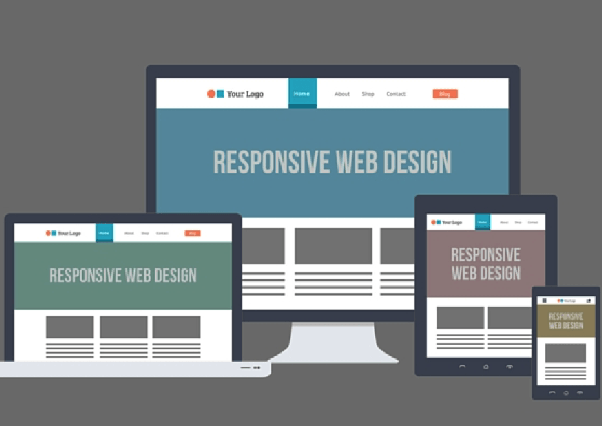
\includegraphics[scale=0.5]{Images/RWD.png}
\caption[Responsive Web Design]{Responsive Web Design \cite{RWD3}}
\end{figure}
\subsection{Asynchronous Javascript (Ajax)}
Ajax stands for Asynchronous Javascript. It’s a combination of several technologies working together in powerful new ways. It allows parts of a web page to be updated without having to reload the entire page \cite{garrett2005ajax}.Ajax incorporates XML or JSON, CSS, Javascript and XMLHttpRequest objects \cite{AJAX}. XML or JSON are text-only format used to transfer data from server to browser script. Developers are increasingly using JSON over XML because of its native JavaScript compatibility. CSS is the language used to style how the data will look on screen. Javascript is used to display the data in the browser and processes user requests/interactions like clicks. XMLHttpRequest objects are the keystone of AJAX, they actually retrieve the data with the server behind the scenes. All modern browsers support XMLHttpRequests. Ajax changed usability and the speed of web applications with its innovative concept: asynchronously exchanging small amounts of data with the server behind the scenes, without affecting the rest of the page \cite{AJAX}.

The classic web application model starts with a user making an action in the interface that triggers an HTTP request back to a web server \cite{garrett2005ajax}. The server does some processing — retrieving data, talking to various systems — and then returns an HTML page to the client. This approach makes a lot of technical sense, but it doesn’t make for a great user experience. While the server is doing the processing, the user is waiting. 

An Ajax application eliminates the start-stop-start-stop nature of interaction on the Web by introducing an intermediary — an Ajax engine — between the user and the server \cite{garrett2005ajax}. When loading a web page, the browser loads an Ajax engine — written in JavaScript and tucked away in a hidden frame. The Ajax engine is responsible for rendering the interface the user sees as well as communicating with the server on the user’s behalf \cite{garrett2005ajax,AJAX}. The user interaction with the server happens asynchronously; the user is never staring at a blank window or a loading icon. Figure 5.2 shows the classic web application model vs the Ajax web application model flows.
\begin{figure}[H]
\centering
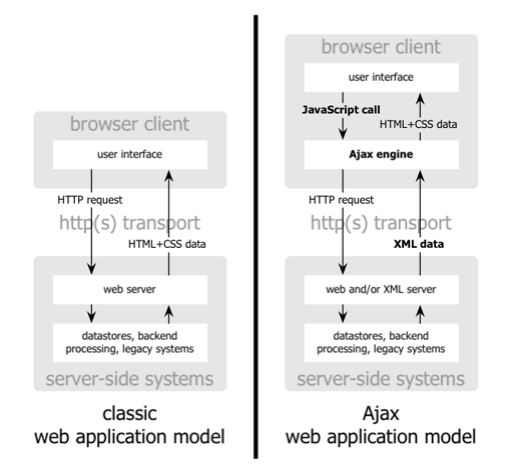
\includegraphics[scale=0.5]{Images/Ajax.png}
\caption[Classic vs Ajax Web Application Model]{Classic vs Ajax Web Application Model \cite{garrett2005ajax}}
\end{figure}
\section{Front-End Technologies}
World Wide Web is always growing and changing. A few years ago the majority of users browsed the web using desktop computers with relatively similar resolutions and dimensions. Internet Explorer was the main browser used for websites browsing; Firefox, Chrome or Opera were less popular \cite{FrontEndSKI}. In the last few years, new devices appeared for example: smart phones, tablets, glasses and even smart TVs. These devices triggered website interfaces evolution \cite{FrontEndSKI}. The interfaces became more complex, dynamic yet stayed user friendly \cite{FrontEndSKI}. Responsive web design approach became a standard and AJAX is broadly used. This evolution led web developers to find a different way to maintain their websites responsiveness, apply code optimizations and develop websites with better performance and scalability \cite{FrontEndSKI}. All these aspect led to the creation of front-end frameworks.

A front-end framework is all what user sees and allows him to use the application. Framework is a platform, foundation on which ready software solutions are built, in this particular case – web interfaces. For this purpose front-end framework consists of ready components, which are used by a developer when working on a project. These components can be modified or adjusted to current needs \cite{FrontEndSKI}.
\subsection{Bootstrap}
Bootstrap is currently the most popular front-end framework. It was created by Mark Otto and Jacob Thornton, developers working in Twitter \cite{FrontEndSKI}. Its main goals included supporting developers for fast development of web applications, having a consisted code, easier maintenance as well as easier further development. Bootstrap allows for rapid, responsive development that is consistent and well supported by the development and design community. It offers ready-made coding blocks which can be utilized to build a website easily. It also has a very short learning curve and is easy to use for beginners in web development. Bootstrap's most important components are \cite{FrontEndSKI}:
\begin{itemize}
	\item \textbf{CSS files:} They contain the global settings that the website should have as well as define the look of the most important HTML items, i.e. text, lists, form elements, tables or images \cite{FrontEndSKI}. The files also comprises of a set of ready-to-use, frequently employed on today’s websites, components. These components include expanding elements, buttons with advanced features (e.g. grouping), navigation menu, paginations, messages or progress bars \cite{FrontEndSKI}.
	\item \textbf{JS files:} They contain ready-to-use plug-ins of popular jQuery libraries. They support creating interfaces with dynamic elements quickly. Most important are components include modals, carousel sliders, dynamic tabs, expandable lists, accordions or tooltips \cite{FrontEndSKI}. Manipulation of these items can be done using HTML attributes rather than Javascript which makes it really special.
\end{itemize}
\subsubsection{Advantages of Bootstrap}
\begin{itemize}
	\item Speed of Development: Bootstrap enables the utilization of ready made blocks of code to help the developers get started instead of writing code from scratch \cite{Bootstrap5}. Bootstrap also supports cross-browser compatibility and CSS-Less functionality, thus saving many hours of development time.
	\item Responsiveness: Bootstrap has a fluid grid layout that dynamically adjusts to the proper screen resolution \cite{Bootstrap5}.
	\item Consistency: Bootstrap ensures consistency regardless of who’s working on the project. In addition, results are uniform across platforms so output remains the same even when using different browsers \cite{Bootstrap5}.
	\item Customizable: Bootstrap can be tailored. Developers can pick and choose the features that are needed and the rest can be tossed. This is easily accomplished using the Bootstrap customize page where the developer can tick the features they need or don't need \cite{Bootstrap5}.
	\item Support: Bootstrap has a huge support community behind it and support can be found for any issues the developer may encounter \cite{Bootstrap5}.
\end{itemize}
\section{Back-End Technologies}
The back-end usually consists of three parts: a server, an application, and a database \cite{Backend}. It is known as the server-side. It is responsible for storing and organizing data, and ensuring everything on the client-side actually works. The back-end communicates with the front-end, sending and receiving information to be displayed as a web page in a website \cite{Backend}.

A website needs a database to manage all it's needed information. A database stores website content in a structure that makes it easy to retrieve, organize, edit, and save data. It runs on a remote computer called a server. There are many different databases that are widely used, such as MySQL, SQL Server, PostgresSQL, and Oracle. A website is built using a language that a database can recognize. Some common back-end languages are Ruby, PHP, Java, .Net, and Python. These programming languages often run on frameworks that simplify the web development process. Spring, for example, is a framework written in Java. 
\subsection{Spring Framework}
Spring is a very popular Java-based framework for building web and enterprise applications \cite{SpringBoot}. Spring framework provides flexibility to configure beans in multiple ways such as XML, Annotations, and JavaConfig which is considered the backbone of a website or an application. Spring boot was created by the spring team to address the complexity of configuration. It is very popular because of several reasons \cite{SpringBoot}:
\begin{itemize}
	\item Spring dependency injection approach encourages writing testable code
	\item Powerful database transaction management capabilities
	\item Integration with other Java frameworks like JPA/Hibernate ORM, Struts/JSF/etc. web frameworks is simplified
	\item Spring utilizes some of the well-known technologies, ORM frameworks, logging frameworks, JEE, JDK timers, Quartz etc., there is no need to re-invent the wheel and developers don’t have to learn any new technologies or frameworks \cite{SpringAdv}
	\item Spring framework provides inversion control and APIs to translate technology-driven exceptions, specifically thrown by JDBC, Hibernate or JDO, into unchecked and consistent ones \cite{SpringAdv}
	\item Due to modularly organized nature, Spring makes it easy for the developers to know which packages or classes are to be used and which one should be ignored \cite{SpringAdv}
	\item With the help of consistent transaction management interface, Spring framework easily scale down or scale up local as well as global transactions\cite{SpringAdv}
	\item Spring Web MVC framework for building web applications is State of the art 
\end{itemize}
\subsubsection{Dependency Injection}
Martin Fowler created Dependency Injection. In object oriented design, objects have relationships with one another \cite{DI}. Dependency Injection design pattern is used to define the object dependencies between each other and try to eliminate it if possible. It exits in two major types Setter Injection and Constructor Injection.

A design based on independent classes / components increases the re-usability and possibility to test the software. A software design based on dependency injection is possible with standard Java. An example to explain DI is as follows:\\
We can have two classes A and B where Class A depends on Class B. DI will inject Class B into Class A by using Inversion of Control (IoC) as shown in figure 5.3 \cite{DI}.
\begin{figure}[H]
\centering
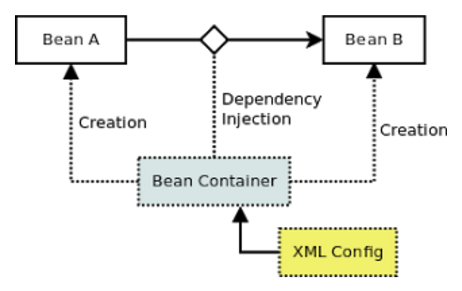
\includegraphics[scale=0.5]{Images/DI.png}
\caption[Dependency Injection]{Dependency Injection \cite{DI}}
\end{figure}
% \subsection{MySQL Database}
% MySQL is the most popular Open Source SQL database management system. It is developed, distributed, and supported by Oracle Corporation \cite{WhatisMySQL}. MySQL is an open source relational database management system (RDBMS) based on Structured Query Language (SQL) \cite{MySQL}. 
\section{System Architecture \& Components}
\label{SystemArchitectureAndCompronents}
In the Following sections, we will discuss how different components of the application were implemented, Why they were implemented in that way and discuss any considerations that were taken during the development process. We will start by discussing the database Design and Implementation followed by the web portal, the decision support and finally the data visualization.
\subsection{Database Design and Implementation}
\label{subsec:DatabaseDesignandImplementation}
In this Section we will discuss the database design and Implementation that was created for our prototype and why we chose to implement it in that way.

As already highlighter, our work is based on the work already implemented in the Connect Hydro project described in \textit{ChapterThree}.In Connect Hydro, a device was added at the power plants which had many ports, each port is connected to a sensor. The sensor data which is the voltage that a sensor is reading at a certain moment is sent to their database. The database was implemented using MySQL and data was sent to it from every device every 10 seconds. Their database consisted of two tables. One included all the sensor data retrieved from the devices in the power plants that were participating in the experiment. The second included the encoding of these sensor values, the factor that should be multiplied to the sensor values in the first table to produce the actual value. The Tables structure they used is shown below.
\begin{figure}[H]
\centering
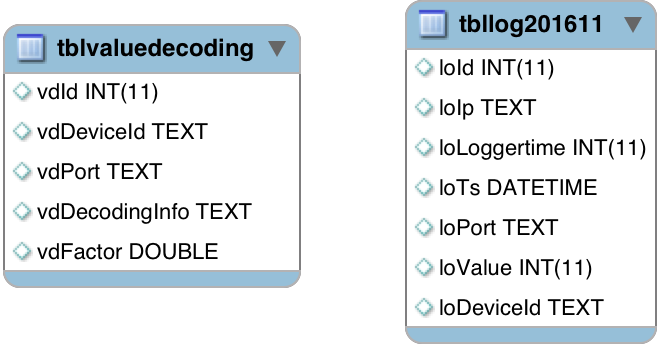
\includegraphics[scale=0.4]{Images/LoggingDatabase.png}
\caption[Connect Hydro Tables]{Connect Hydro Tables}
\end{figure}
The following table explains what each column in the database table tbllog201611 represented.
\begin{center}
\begin{tabular}{ |c|c| } 
 \hline
 Column Name & Explanation\\ [0.5ex] 
 \hline\hline
loId & Id, Primary Key\\ 
\hline
loIP & IP-Address of the Loggers at the power plant (Not Unique, always changing)\\ 
\hline
loLoggerTime & Time of when the data was collected at the power plant\\ 
\hline
loTs & Timestamp of when the value was inserted into the DB\\ 
\hline
loPort & Port ID of the device that is sending the value\\ 
\hline
loValue & Raw value collected by the device from the sensor\\
\hline
loDeviceId & Device ID that this sensor data is collected from (Unique)\\
 \hline
\end{tabular}
\end{center}
The columns in the tblvaluedecoding are explained in the following table.
\begin{center}
\begin{tabular}{ |c|p{10cm}| } 
 \hline
 Column Name & Explanation\\ [0.5ex] 
 \hline\hline
vdId & Id, Primary Key\\ 
\hline
vdDeviceId & Device ID that this sensor data is collected from (Unique)\\
\hline
vdPort & Port ID of the device that is sending the value\\ 
\hline
vdDecodingInfo & Any extra information (Always NULL)\\
\hline
vdFactor & The factor that should be multiplied to the raw value in the previous table to get the actual value\\ 
 \hline
\end{tabular}
\end{center}
As shown above the connect hydro database was not well structured, In our thesis a new database design is proposed and implemented. The database design was created not only to fit the connect hydro project scope but took into consideration that it can be implemented in other locations in the future. It included information about power plants, their operators, the river that the power plant are located on. Information about Devices installed at the power plants, their ports, the connected sensors and any rules the operators defined were also included. 

There were two main focuses for the database; The Power Plants and the Devices; each will be discussed separately but their relation will be clearly defined. In the rest of this section we will discuss the new database design and the relations created between the different tables.

In our scope, a power plant was defined as a location which had its own water supply (water channel) and had a power output turbine. The information collected about power plants were its name, geographical coordinates, distance between its predecessor and successor power plants. It was also given a unique ID. Multiple operators could operate one power plant. Data collected about operators included their name, Email, phone number, address and each operator was also assigned a unique ID. As Many power plants are located along the same river, that relation was also included and each river was identified by a unique ID as well as its name, Length and any other description the system admin wanted to include. The above relations are demonstrated in figure 5.5.
\begin{figure}[H]
\centering
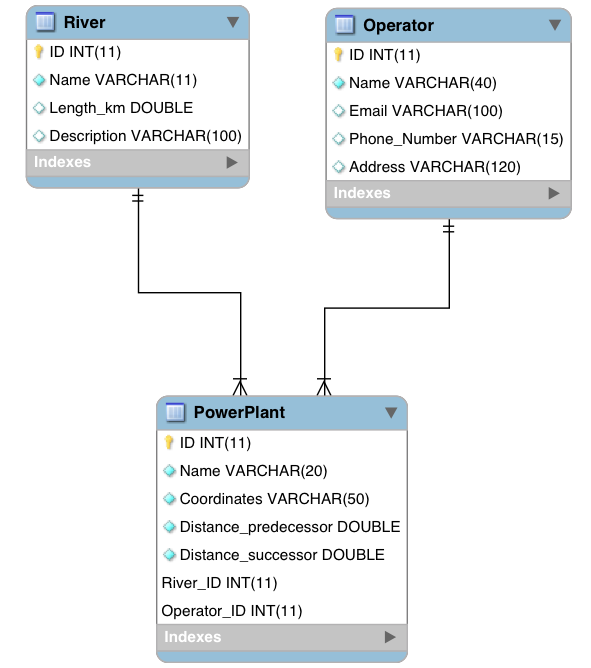
\includegraphics[scale=0.4]{Images/PP_River_Operator.png}
\caption[Power Plant-Operator-River Relation]{Power Plant-Operator-River Relation}
\end{figure}
Each of the three power plants that participated in the connect hydro project was fitted with a device. This device was created by NEXTSOFT IT GMBH in a contribution to the connect hydro project. It is a piece of hardware that is installed at the power plants. In some cases, one device can collect data from more than one power plant.
\begin{figure}[H]
\centering
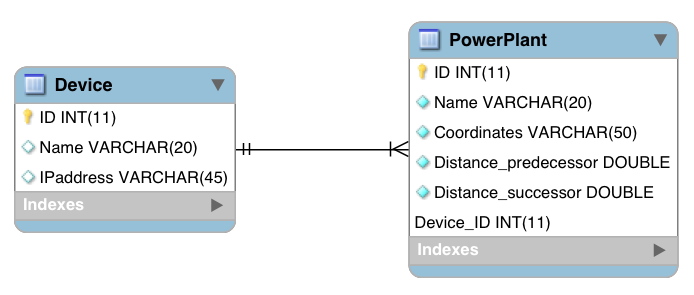
\includegraphics[scale=0.4]{Images/Device-Powerplant.png}
\caption[Power Plant-Device Relation]{Power Plant-Device Relation}
\end{figure}
A device is identified by its unique ID and Name; an IP address is also included in the device table but it changes frequently. A device includes multiple ports and each port is connected to a sensor. Each port in the same device has a unique name. 
\begin{figure}[H]
\centering
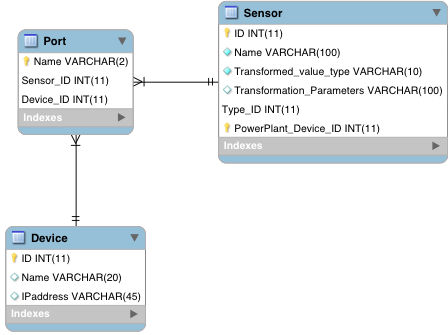
\includegraphics[scale=0.6]{Images/Device-Port-Sensor.png}
\caption[Device-Port-Sensor Relation]{Device-Port-Sensor Relation}
\end{figure}
Each Sensor had the following specifications: Unique ID, Name, variables indicating the transformed value type and parameters and a sensor type. The transformed value parameters maps the vdFactor in the original connect hydro database. The transformed value type is added to handle future situations where a transformed value is not just a numeric value but a percentage or anything else. As already mentioned each sensor has a type, all the sensor types are added in a separate table and is referenced from the sensors table. The power plant operators can add rules specific to every sensor in their power plant that are processed and evaluated later in the decision support module. These rules are specified in a separate table as well and are identified by a name and parameter/s.
\begin{figure}[H]
\centering
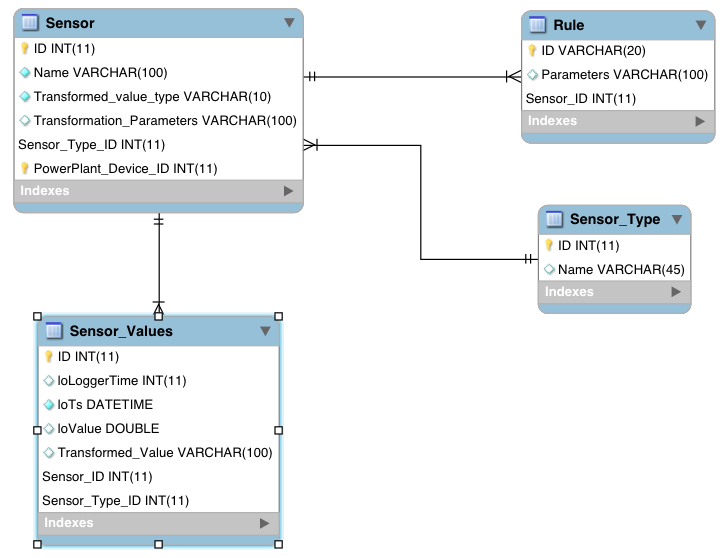
\includegraphics[scale=0.5]{Images/SensorRelations.png}
\caption[Sensor Relations]{Sensor Relations}
\end{figure}
The sensor Values table is the table that maps the data in the tbllog201611 to our database. It contains some columns with the same names as the original table like loLoggerTime, loTs and loValue. It also contains the Transformed\_Value column which is the raw value (loValue) multiplied by the transformation parameters.

The database included some other tables that were not connected any tables. They included a table saving the relation between two successor power plants, a table saving all the emails and passwords of the users who will use the web portal and finally a table with Actions and warnings messages to the power plant operators; its function will be discussed later.
\begin{figure}[H]
\centering
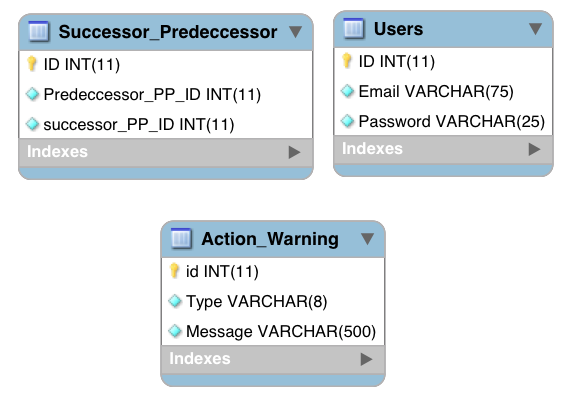
\includegraphics[scale=0.5]{Images/Othertables.png}
\caption[Separate Tables]{Separate Tables}
\end{figure}
For the scope of our project, we extracted one month data from the original connect hydro database and using a series of manual SQL queries added them into our database. We chose September 2016 for the demo data as it highlighted a few interesting events which were later used for the decision support and the data visualization. The Data extracted corresponding to that month included 1062321 records. An example query used is:\\
\begin{center}
\begin{verbatim}
INSERT INTO `Sensor_Values` 
( loLoggerTime, loTs, loValue, Transformed_Value, Sensor_ID, Sensor_Type_ID) 
SELECT loLoggertime, loTs, loValue , '1', 1, 2 
FROM `tbllog201611` 
WHERE loDeviceId = 'Lippenannerl' AND loPort = 'a0' OR loPort = 'A0' ;
\end{verbatim}
\end{center}
\subsection{Web Portal}
A web portal was developed for our prototype in this thesis. It included a connection to the database, the decision support system module and the data visualization. For our development we chose Spring MVC framework mainly because it's flexibility and ease of integrating all the technologies we use in it. It is based on Java which was the preferred language for the connect hydro team.

The first functionality that was implemented in the portal was the sign in. 
\subsection{Decision Support}
\label{subsec:DecisionSuport}
\subsection{Data Visualization}
\label{subsec:DataVisualization}